\documentclass{standalone} % run wit shell escape

\usepackage{tikz}
\usetikzlibrary{arrows}
\usepackage{verbatim}
\usepackage{amsmath}

\usepackage{tikz}
\usepackage{color}
\definecolor{honeydew}{rgb}{0.94, 1.0, 0.94}
\definecolor{ivory}{rgb}{1.0, 1.0, 0.94}
\usetikzlibrary{shapes,arrows}
\tikzstyle{block} = [draw, fill=honeydew!70, rectangle, line width=0.5mm,
    minimum height=3em, minimum width=5em]
\tikzstyle{sum} = [draw, fill=ivory!20, circle, node distance=1cm, line width=0.5mm]
\tikzstyle{input} = [coordinate]
\tikzstyle{output} = [coordinate]
\tikzstyle{pinstyle} = [pin edge={to-,thick,black}]

\tikzset{
    circ/.style={draw, circle, fill=ivory!70}
}


\begin{document}
% The block diagram code is probably more verbose than necessary
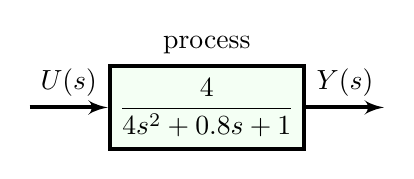
\begin{tikzpicture}[auto, node distance=1cm,>=latex']
    \node [block, node distance=1.75cm, label=process] (g) {$\dfrac{4}{4s^2+0.8s+1}$};
    \node [input, node distance=2.25cm, left of=g] (U) {};
	\node [output, name=output, right of=g, node distance=2.25cm] {$Y(s)$};
	
    \draw [->, line width=0.5mm] (U) -- node {$U(s)$} (g);
    \draw [->, line width=0.5mm] (g) -- node {$Y(s)$} (output);
\end{tikzpicture}

\end{document}
